\section{Durchführung}
\label{sec:Durchführung}

\subsection{Vorbereitung}
Ein Diodenlaser, sowie eine Absorptionszelle mit Rubidium sind
auf einem Optischen Tisch befestigt.
Der Diodenlaser ist mit einem Netzgerät mit Reglern für
Temperatur, Stromeinstellung und weiteren Einstellmöglichkeiten
verbunden, um den für die Rubidiumabsorptionslinien notwendigen Wellenlängenbereich abzudecken.
Des weiteren kann am Diodenlaser mithilfe eines sechskantigen
Winkelschraubendrehers das Beugungsgitter horizontal, wie auch vertikal verstellt werden.
Mit dem Controller wird der Laser auf die Betriebstemperatur von $\qty{50}{\degreeCelsius}$ erhitzt.
Für den weiteren Aufbau sind verschiedene Linsen, ein $50 / 50$-Strahlteiler
und eine CCD-Kamera, um das nicht sichtbare Infrarot-Licht sichtbar zu machen, notwendig.
Außerdem wird der Raum abgedunkelt.

\subsection{Schwellenstrom}
\label{subsec:Schwelle}
Im folgendem Versuchsteil wird der Schwellenstrom mithilfe der Lasergranulation bestimmt.
Diese tritt auf sobald der Laser den LED-Bereich verlässt.
Der Aufbau wird gemäß Abbildung \ref{pic:aufbau} realisiert. 
\begin{figure}
    \centering
    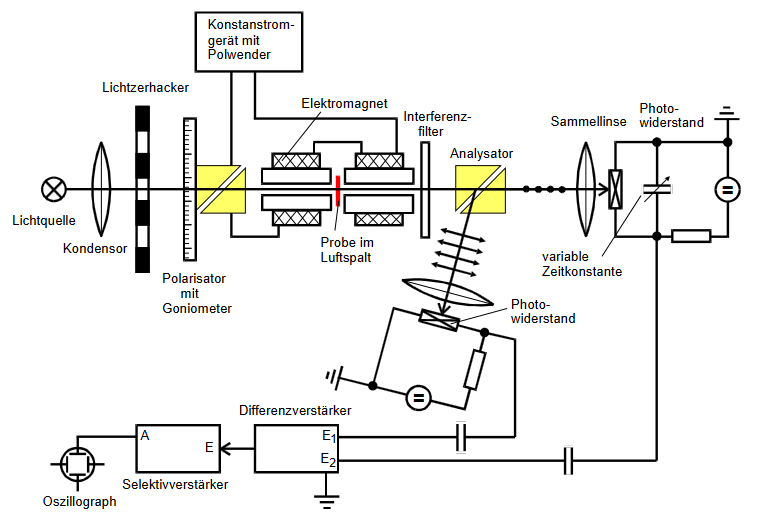
\includegraphics[width = 0.78\textwidth]{pictures/aufbau.png}
    \caption{Verwendeter Aufbau zur Bestimmung des Schwellenstroms\cite{anleitung}}
    \label{pic:aufbau}
\end{figure}
Am Laser wird das Gitter bei minimalem Strom soweit verstellt, dass an der Detektorkarte Licht sichtbar wird.
Der Strom wird dann langsam erhöht, bis Lasergranulation auftritt.
Daraufhin wird der kleinste Wert bei dem Lasergranulation sichtbar wird, als Schwellenstrom notiert.

\subsection{Rubidiumfluoreszenz und Absorptionsspektrum}
Um die Rubidiumfluoreszenz sichtbar zu machen werden die Absorptionszelle und einige Filter in den Verlauf des Laserstrahls eingebaut.
Für das Absorptionsspektrum können auch schon der $50 / 50$-Strahlteiler, so wie die Photodioden wie in Abbildung
\ref{pic:Absorptionsspektrum} eingebaut werden. Außerdem wird ein Oszilloskop mit dem Controller verbunden um das Spektrum später sichtbar zu machen.
Der Strom wird weit über den Schwellenstrom eingestellt und die CCD-Kamera wird auf die Rubidiumzelle gerichtet.
Im folgenden wird das Gitter am Laser verstellt, so dass die Fluoreszenz in der Rubidiumzelle
erkennbar wird. Durch feine veränderungen am Piezo Controller, am Strom und am Gitter wird die durch die CCD-Kamera
sichtbare Fluoreszenz maximiert, so dass ein stabiler Strahl entsteht, welcher dann abfotographiert wird.
\begin{figure}
    \centering
    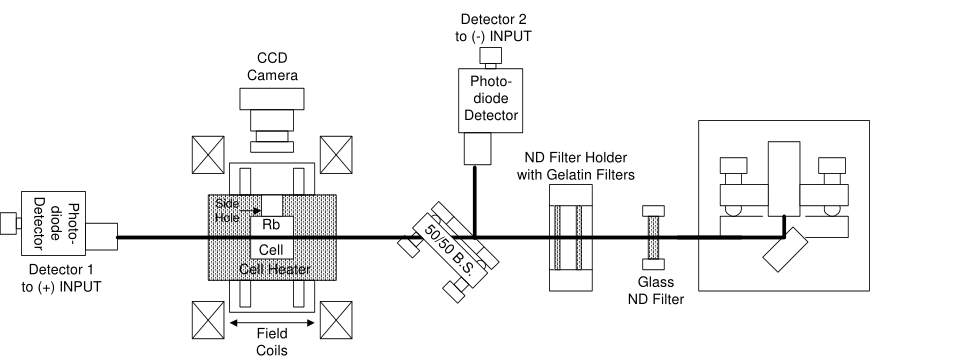
\includegraphics[width = 0.78\textwidth]{pictures/Aufbau_abs.png}
    \caption{Aufbau für die Aufnahnmen der Rubidiumfluoreszenz und Absorptionsspektren\cite{anleitung}}
    \label{pic:Absorptionsspektrum}
\end{figure}
Für den letzten Versuchsteil werden die Photodioden an den Controller und über diesen mit
dem Oszilloskop verbunden, sodass eine Unterdrückung des Untergrunds sichtbar wird. Nun erfolgt eine Feinjustierung um Modensprünge, welche das Absorptionsspektrum verzerren, zu verhindern.
Nach dem Justieren kann das auf dem Oszilloskop entstandende Bild abfotographiert werden.